\documentclass[10pt,aspectratio=169]{beamer}

\usetheme{metropolis}           % Use metropolis theme
\title{GFS Mathematik Lineare Algebra}
\date{20. Januar 2023}
\author{Valentin Zwerschke}
\institute{Königin-Olga-Stift Gymnasium}

\def\titlepage{%
  \usebeamertemplate{title page}%<---
}

\graphicspath{ {./images/} }

\usepackage{tikz}
\usepackage[german]{babel} % German

\begin{document}
  \maketitle

  \begin{frame}{Gliederung}
	\setbeamertemplate{section in toc}[sections numbered]
	\setbeamertemplate{subsection in toc}[subsections numbered]
	\tableofcontents[hideallsubsections]
  \end{frame}

  \section{Vektoren}
  \subsection{Vektoren}
  \begin{frame}{Vektoren}
    \begin{minipage}{0.65\textwidth}
      \begin{itemize}
        \item Punkte im Raum werden ueber Vektoren beschrieben 
        \item Vektor Koordinaten $v_x$ und $v_y$ (Kartesischem Koordinaten System = Achsen Senkrecht)\\\vspace{0.2cm} 
        \hspace{0.3cm}$\vec{v} = \begin{pmatrix} v_x\\ v_y\end{pmatrix}$
        \vspace{0.2cm}
        \item Laenge (euklidische Norm) bsp. 2D, 3D\\
        \hspace{0.3cm}$||\vec{v}|| =  \sqrt{v_x^2 + v_y^2}$\\
        \hspace{0.3cm}$||\vec{v}|| =  \sqrt{v_x^2 + v_y^2 + v_z^2}$
        \vspace{0.2cm}
        \item Richtung/Normierter Vektor\\
        \hspace{0.25cm}\Large$\frac{\vec{v}}{||\vec{v}||}$
      \end{itemize}  
    \end{minipage}
    \begin{minipage}[c]{0.3\textwidth}
      \begin{tikzpicture}
        \draw[thick,->] (0,0) -- (3.5,0) node[anchor=north west] {x};
        \draw[thick,->] (0,0) -- (0,2.5) node[anchor=south east] {y};
        \draw[thick,->, blue] (0,0) -- node[above] {$\vec{v}$} (3,2) node[anchor=north east] {};
        \draw[densely dotted]  (3,0) node[below] {$v_x$} -- (3,2);
        \draw[densely dotted]  (0,2) node[left] {$v_y$} -- (3,2);
        %\node [black] at (3,2) {\textbullet};
      \end{tikzpicture}
    \end{minipage}
  \end{frame}

  \subsection{Rechnen mit Vektoren}
  \begin{frame}{Rechnen mit Vektoren}
    \vspace{0.2cm}
    \begin{minipage}{7cm}
      \textbf{Addition}
      \begin{itemize}
        \item Jeweils Summe der Koordinaten\\
        \vspace{0.2cm}
        \hspace{0.2cm}
        $\vec{u} + \vec{v} = \begin{pmatrix}u_x + v_x\\ u_y + v_y\end{pmatrix}$
        \vspace{-0.5cm}
      \end{itemize}
      \hspace{0.25cm}
      \begin{tikzpicture}
        \draw[thick,->] (0,0) -- (3.5,0) node[anchor=north west] {x};
        \draw[thick,->] (0,0) -- (0,2.5) node[anchor=south east] {y};

        \draw[thick,->, blue] (0,0) -- node[above] {$\vec{u}$} (3,1);
        \draw[thick,->, blue] (3,1) -- node[above] {$\vec{v}$} (1.5,2);
        \draw[thick,->, red]   (0,0) -- node[above] {\hspace{1.4cm}\small$\vec{u} + \vec{v}$} (1.5,2);
      \end{tikzpicture}
    \end{minipage}
    \begin{minipage}{6.5cm}
      \textbf{Subtraktion}
      \begin{itemize}
        \item Jeweils Differenz der Koordinaten\\
        \vspace{0.2cm}
        \hspace{0.2cm}
        $\vec{v} - \vec{u} = \begin{pmatrix}v_x - u_x\\ v_y - u_y\end{pmatrix}$
        \vspace{-0.5cm}
      \end{itemize}
      \hspace{0.25cm}
      \begin{tikzpicture}
        \draw[thick,->] (0,0) -- (3.5,0) node[anchor=north west] {x};
        \draw[thick,->] (0,0) -- (0,2.5) node[anchor=south east] {y};

        \draw[thick,->, blue] (0,0) -- node[above] {$\vec{u}$} (3,1);
        \draw[thick,->, red] (3,1) -- node[above] {\hspace{0.5cm}\small$\vec{v} - \vec{u}$} (1.5,2);
        \draw[thick,->, blue]   (0,0) -- node[above] {$\vec{v}$} (1.5,2);
      \end{tikzpicture}
    \end{minipage}
    \textbf{Skalierung}
    \begin{center}
      $\lambda \vec{v} = \begin{pmatrix}\lambda v_x\\ \lambda v_y\end{pmatrix}$
    \end{center}
  \end{frame}


  \subsection{Skalarprodukt}
  \begin{frame}{Skalarprodukt}
    \begin{minipage}{9cm}
      \begin{itemize}
        \item Abbildung zweier Vektoren auf einen Skalar (Zahl)
        \item Skalarprodukt:\\
        $\vec{u}\cdot\vec{v} = u_xv_x + u_yv_y$; im 2D\\
        $\vec{u}\cdot\vec{v} = u_xv_x + u_yv_y + u_zv_z$; im 3D\\
        \item Winkel zwischen $\vec{u}$ und $\vec{v}$:\\
        \hspace{0.7cm}$\vec{u} \cdot \vec{v} = \cos(\phi)||\vec{u}||||\vec{v}||$
        \item Orthogonlaitaet genau dann wenn:
        \hspace{0.7cm}$\vec{v} \perp \vec{u} \Leftrightarrow \vec{u} \cdot \vec{v} = 0$
        \item Orthogonale Vektoren zu $\vec{v}$:\\
        \vspace{0.1cm}\hspace{0.7cm}$\lambda \small\begin{pmatrix}v_y\\ -v_x\end{pmatrix}$, \small mit $\lambda \neq 0$
      \end{itemize}
    \end{minipage}
    \begin{minipage}{4cm}
      \textbf{Interpretation}\\
      \footnotesize Produkt Laenge $\vec{u}$ mit Laenge Projektion von $\vec{v}$ auf $\vec{u}$ (hier: $s$)\\
      \vspace{0.1cm}
      \begin{tikzpicture}
        \draw[thick,->] (0,0) -- (3.5,0) node[anchor=north west] {x};
        \draw[thick,->] (0,0) -- (0,2.5) node[anchor=south east] {y};
        \draw[thick,->] (0.5,0.5) -- node[above] {$\vec{v}$} (2,2);
        \draw[thick,->] (0.5, 0.5) -- node[above] {$\vec{u}$} (3,0.5);
        \draw[thick,<->, blue] (0.5, 0.35) -- node[below] {$s$} (2,0.35);
        \draw[densely dotted]  (2,0.5) -- (2,2);
        
      \end{tikzpicture}
    \end{minipage}
  \end{frame}

  \subsection{Kreuzprodukt}
  \begin{frame}{Kreuzprodukt}
    \begin{minipage}{10cm}
      \begin{itemize}
        \item Abbildung zweier Vektoren $\vec{u}$ und $\vec{v}$ im 3D Raum auf einen Vektor $\vec{w}$\\\vspace{0.25cm}
        \hspace{0.3cm}$\vec{w} = \vec{u} \times \vec{v} = \begin{pmatrix}u_x\\ u_y\\u_z\end{pmatrix} \times \begin{pmatrix}v_x\\v_y\\v_z\end{pmatrix} = \begin{pmatrix}u_yv_z - u_zv_y\\u_zv_x - u_xv_z\\u_xv_y - u_yv_x\end{pmatrix}$ 
        \vspace{0.25cm}
        \item Eigenschaften:
        \begin{itemize}
          \item $\vec{w} \perp \vec{u}$ \hspace{0.1cm}$\wedge$\hspace{0.1cm} $\vec{w} \perp \vec{v}$ ("Rechte Hand Regel")
          \item $||\vec{w}|| = ||\vec{u}||||\vec{v}||\sin(\phi)$, mit $\phi$ Winkel zwischen $\vec{u}$ und $\vec{v}$\\
          Entspricht der Flaeche, des von $\vec{u}$ und $\vec{v}$ aufgespannten Parallelogramms
        \end{itemize}
      \end{itemize}  
    \end{minipage}
    \begin{minipage}{3cm}
      \begin{tikzpicture}
        \draw[thick,->] (0,0) -- (3.5,0) node[anchor=north west] {x};
        \draw[thick,->] (0,0) -- (0,2.5) node[anchor=south east] {y};

        \draw[thick,->, blue] (0.5,1) -- node[above] {$\vec{v}$} (1.5,2);
        \draw[thick,->, blue] (0.5,1) -- node[below] {$\vec{u}$} (2.5,0.5);
        
        \draw[thick, magenta] (1.5,2) -- (3.5,1.5);
        \draw[thick, magenta] (2.5,0.5) -- (3.5,1.5);

        \node [black] at (2,1.25) {\small$||\vec{u} \times \vec{v}||$};
      \end{tikzpicture}
    \end{minipage}
  \end{frame}

  \section{Polygonale Netze}
  \subsection{Vertex, Kante, Facette, Oberflaeche}
  \begin{frame}{Vertex, Kante, Facette, Oberflaeche}
    \hspace{0.65cm}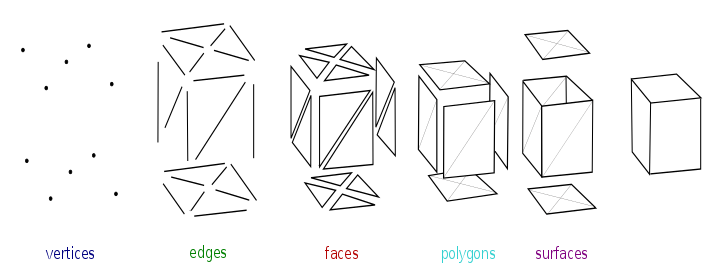
\includegraphics[scale=0.5]{mesh}
    \begin{center}
      \footnotesize \url{https://commons.wikimedia.org/wiki/File:Mesh_overview.svg}  
    \end{center}
  \end{frame}

  \subsection{Beispiel einer Oberflaeche}
  \begin{frame}{Beispiel einer Oberflaeche}
    \begin{center}
      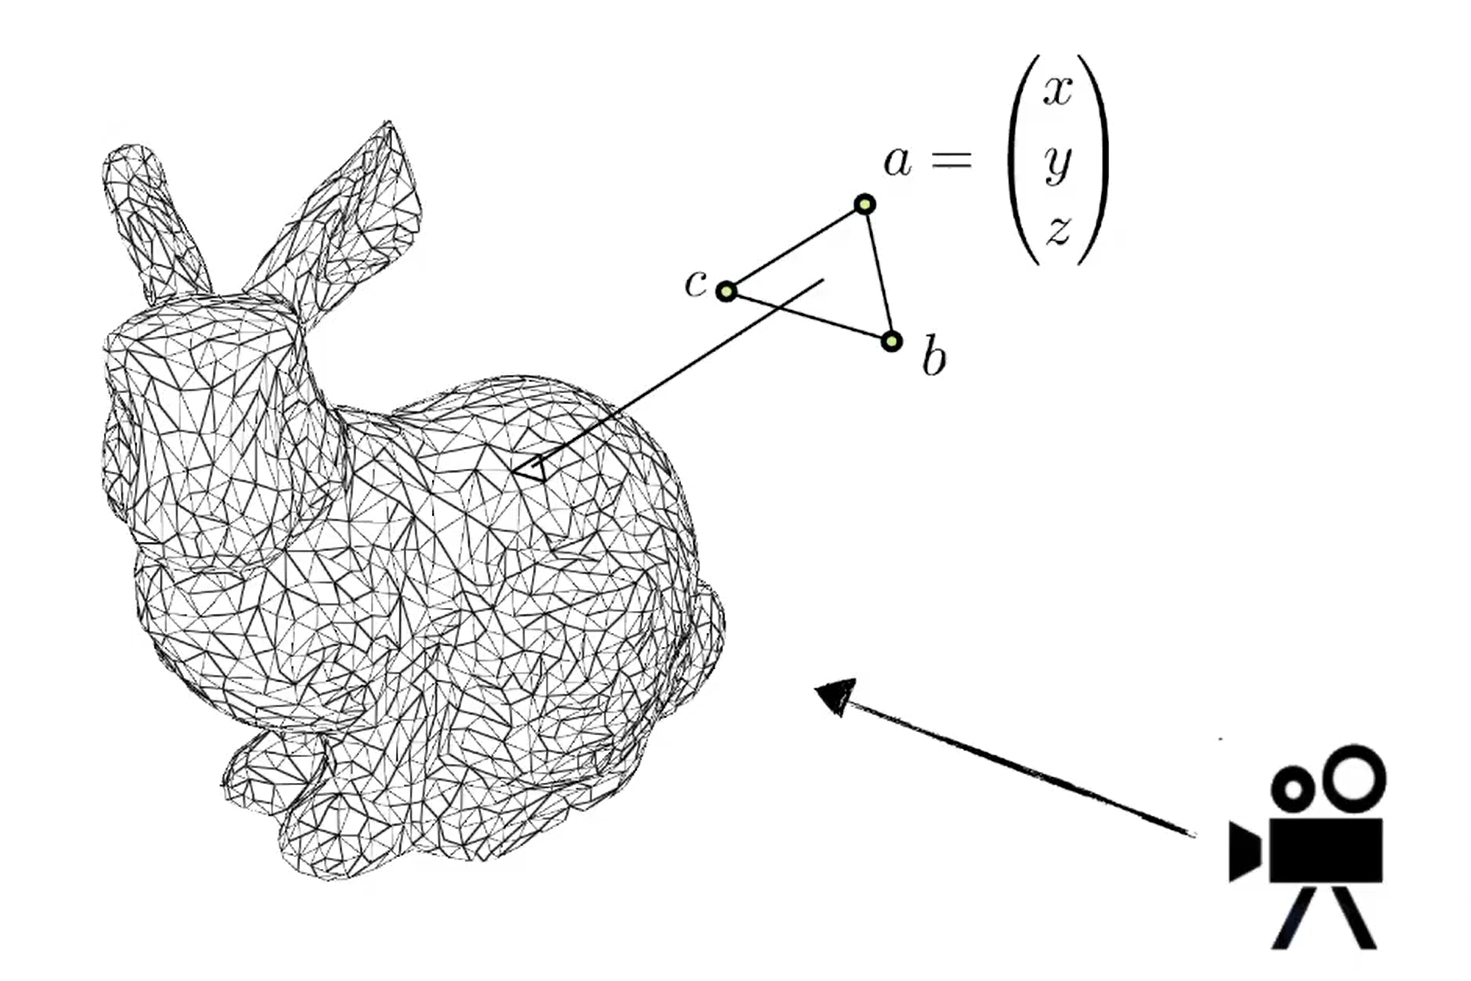
\includegraphics[scale=0.125]{bunny}
    \end{center}
    \textbf{Fragestellung der Computergrafik:}\\
    Abbildung der 3D Oberflaeche auf die 2D Bildebene der Kamera\\
    (Kameraperspektive, Schattierung, ... )
  \end{frame}


  \subsection{Flaechennormale}
  \begin{frame}{Flaechennormale}
    \begin{minipage}{8cm}
      \normalsize
      \textbf{Der Normalenvektor zu einer Facette:}
      \begin{itemize}
        \item Senkrecht zur Facette mit Laenge 1
        \item Wichtig, z.B. fuer Schattierungsberechnung
        \item Berechnung aus der Ortsvektoren, $\vec{a}, \vec{b}, \vec{c}$ der Vertices
        \item Kreuzprodukt der Richtungsvektoren $\vec{u}$ und $\vec{v}$
      \end{itemize}
      
      \vspace{0.2cm}
      \hspace{0.3cm}
      \large $\vec{n} = \frac{\vec{u} \times \vec{v}}{||\vec{u} \times \vec{v}||} = \frac{(\vec{b} - \vec{a}) \times (\vec{c} - \vec{a})}{||(\vec{b} - \vec{a}) \times (\vec{c} - \vec{a})||}$  
    
      
    \end{minipage}
    \begin{minipage}{4cm}
      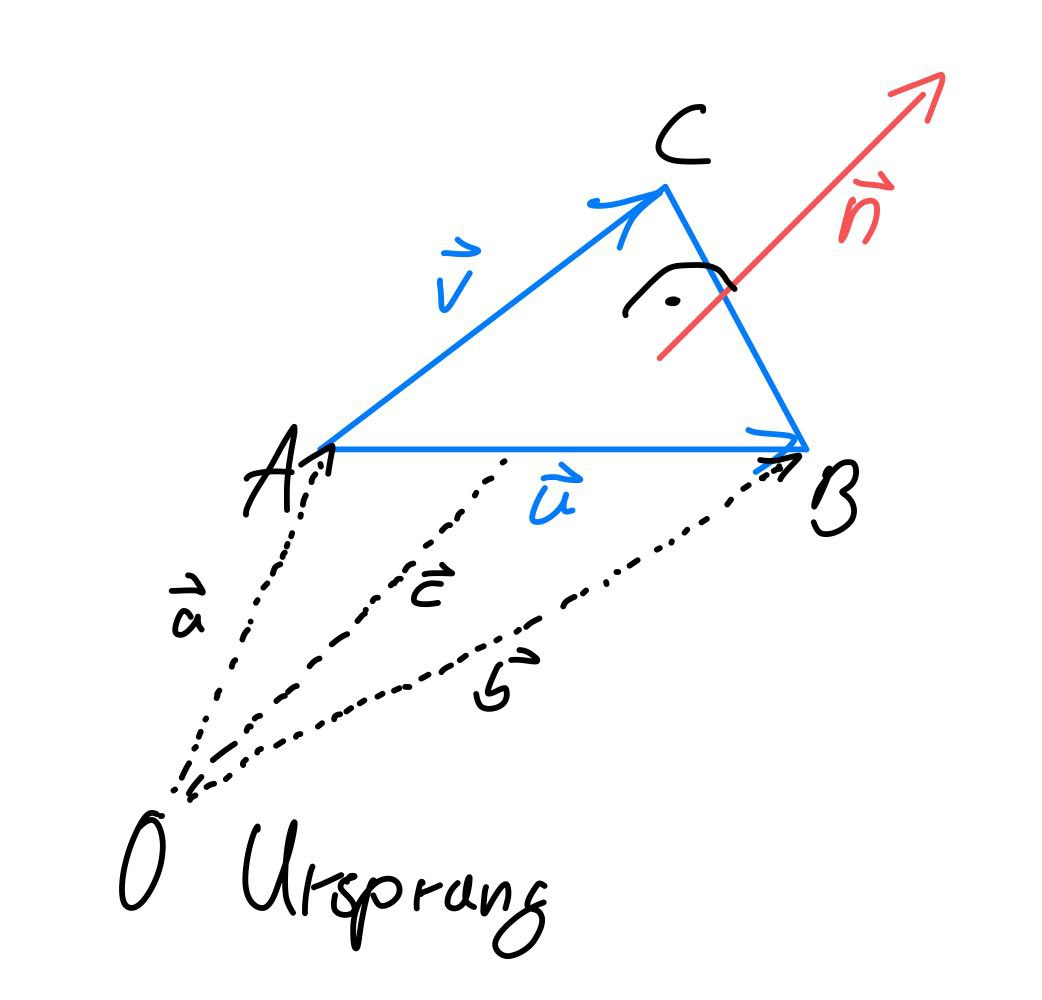
\includegraphics[scale=0.125]{sketch_n_vec}  
    \end{minipage}
   
  \end{frame}


  \subsection{ggf. Gerade und Ebene in Vektorform}
  \begin{frame}{ggf. Gerade und Ebene in Vektorform}
  \end{frame}

  \section{Matrizen}

  \subsection{Defintion und lsg LGS}
  \begin{frame}{Definition und lsg LGS}
  \end{frame}

  \section{Transformation}

  \subsection{Affine Transformation: Skalierung und Rotation}
  \begin{frame}{Affine Transformation: Skalierung und Rotation}
  \end{frame}

  \subsection{Translation, homogene Koordinaten}
  \begin{frame}{Translation, homogene Koordinaten}
  \end{frame}

  \section{Anwendung auf Computer Grafik}


  \subsection{Perspektivische Projektion}
  \begin{frame}{Perspektivische Projektion}
  \end{frame}


  \subsection{Screen Mapping}
  \begin{frame}{Screen Mapping}
  \end{frame}

  \subsection{Abbildung eines Drehbaren Dreiecks im Raum}
  \begin{frame}{Abbildung eines Drehbaren Dreiecks im Raum}
  \end{frame}

\end{document}